\documentclass[psamsfonts]{amsart}

%-------Packages---------
\usepackage{amssymb,amsfonts}
\usepackage[all,arc]{xy}
\usepackage{enumerate}
\usepackage[margin=1in]{geometry}
\usepackage{amsthm}
\usepackage{theorem}
\usepackage{verbatim}
\usepackage{framed}
\usepackage{tikz}
\usetikzlibrary{shapes,arrows}

\newenvironment{sol}{\vspace{0.25cm}{\large \bfseries Solution:}}{\qedsymbol}
\newenvironment{prob}[1]{\begin{framed}{\large \bfseries Problem #1:}}{\end{framed}}
\newcommand{\makenewtitle}{
    \begin{center}
    {\huge \bfseries 6.854 Advanced Algorithms} \\
    Problem Set 2\\
    \vspace{0.25cm}
    {\bfseries John Wang} \\
    Collaborators: Jason Hoch
    \end{center}
    \vspace{0.5cm}
}


\bibliographystyle{plain}

\voffset = -10pt
\headheight = 0pt
\topmargin = -20pt
\textheight = 690pt

%--------Meta Data: Fill in your info------
\title{6.854 \\
Advanced Algorithms \\
Problem Set 4}

\author{John Wang}

\begin{document}

\maketitle

Collaborators: 

\begin{prob}{1-a}
Consider a second-level table, that in the static case uses $f(s) = O(s^2)$ space to store $s$ items. We gave a construction of such a table that succeeds with probability $1/2$. Suppose that we take the following approach to insertions: if inserting the $s$th item violates perfection of the table, repeatedly build a table of size $f(2s)$ until you get a perfect one. Show that when $s$ items are inserted (one at a time, with rebuilds as necessary) the expected total cost of all the rebuilds is $O(s)$. 
\end{prob}

\begin{sol}
Let us examine the insertion cost of a table when we attempt to insert $k$ items in a table of size $k^2$. The probability of collision of the $i$th element inserted is $i/k^2$ since there are $k^2$ different bins. Notice that since $i \leq k$, we can upper bound this probability by $1/k$. Since there are $k$ insertions, the expected number of collisions is $k/k = 1$. Notice that if there is a collision, then we will have to rebuild the table. Therefore, upon inserting $k$ items, we expect to have a single collision. A table rebuild of size $2k$ will require $2k$ time to build and insert all of the elements. 

Thus, if we start our table at size $2$ and we have a series of $s$ insertions, then we will expect to rebuild the table after every $2^i$ insertions for $i \in \{1,2, \ldots, \lg s\}$. Each of these table rebuilds requires $2* 2^i = 2^{i+1}$ time. Therefore, the total cost is given by
\begin{eqnarray}
\sum_{i=1}^{\lg s} 2^{i+1} = 2^{\lg s + 2} = 4* 2^{\lg s} = O(s)
\end{eqnarray}

Therefore, we see that the total expected cost of all the rebuilds is $O(s)$, just as we wanted to show.
\end{sol}

\begin{prob}{1-b}
Let $s_i$ be the number of items in bucket $i$ in the second level table. Make a similar modification for the top level: any time the table on $n$ items has bucket sizes $s_i$ violating the requirement that $\sum s_i^2 = O(n)$, we rebuild the top table and all the second level tables. Show the expected total time is $O(n)$ when $n$ items are inserted.
\end{prob}
\begin{sol}

\end{sol}

\begin{prob}{1-c}
Now consider deletions. When an item is deleted, we can simply mark it as deleted without removing it (and if it reinserted, unmark the deletion). This makes deletion cheap. But if there are many deletions, the table might end up using much more space than it needs, which could mess up the amortized bounds of the previous parts. To fix this, we can rebuild the hash table any time the number of holes (items marked deleted) exceeds half the total items in the table. Show that this cleanup works does not change (can be charged against) the aortized $O(1)$ cost of insertions.
\end{prob}
\begin{sol}
\end{sol}

\newpage 
\makenewtitle

\begin{prob}{2-a}
In any maximum flow, and for all vertices $v$ and $w$, either the raw flow from $v$ to $w$ or the raw flow from $w$ to $v$ is 0.
\end{prob}
\begin{sol}
False. Consider the following graph.

\begin{figure}[h!]
\centering
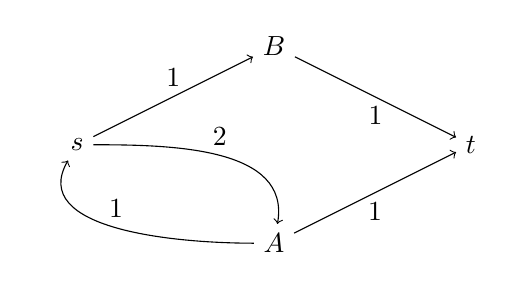
\begin{tikzpicture}[scale=2.5]
\node (s) at (0,0.5) {$s$};
\node (A) at (1,0) {$A$};
\node (B) at (1,1) {$B$};
\node (t) at (2,0.5) {$t$};
\path[->,font=\scriptsize,>=angle 90];
\draw (s) edge [->,relative=false,in=80,out=0] node[above]{2} (A)
(A) edge [->,relative=false,in=-120,out=-180] node[above]{1} (s)
(s) edge [->] node[above]{1} (B)
(B) edge [->] node[below]{1} (t)
(A) edge [->] node[below]{1} (t);
\end{tikzpicture}
\end{figure}

It is clear that the maximum flow is 2, where flow comes into $t$ from nodes $A$ and $B$, each with a flow of 1. However, we can see that there is non-zero raw flow from $s$ to $B$ and from $B$ to $s$. Thus, there is a maximum flow where there exist two vertices $v$ and $w$ which break the above conjecture.
\end{sol}

\begin{prob}{2-b}
There always exists a maximum flow such that, for all vertices $v$ and $w$, either the raw flow from $v$ to $w$ or the raw flow from $w$ to $v$ is zero.
\end{prob}

\begin{sol}
True. We will show this by contradiction. Suppose this is not the case. Then there is raw flow such that on some vertices $v$ and $w$, the raw flow from $v$ to $w$ and from $w$ to $v$ are nonzero for all flows which are maximal. This means that any flow with zero raw flow in each direction is not a maximum flow (of flow $f$), so that this new flow would be less than $f$. Now, consider what happens when we set the raw flow from $w$ to $v$ to be zero, and the raw flow from $v$ to $w$ to be $rf(v,w) - rf(w,v)$ where $rf$ denotes raw flow. In this way, we have created a graph $G'$ which has the same amount of flow as before towards the sink (if not, the switch $v$ and $w$) as in the original graph. This means that the new flow is also a maximum flow. However, we know that the flow on the vertices of the rest of the graph are unchanged, and we also assumed that there does not exist any maximum flow with zero raw flow between any vertices $v$ and $w$. This is a contradiction.
\end{sol}

\begin{prob}{2-c}
If all directed edges in a network have distinct capacities, then there is a unique maximum flow.
\end{prob}

\begin{sol}
False. Consider the following counterexample.
\begin{figure}[h!]
\centering
\begin{tikzpicture}[scale=2.5]
\node (v0) at (0,0) {$s$};
\node (v1) at (1,0) {$A$};
\node (v2) at (3,0) {$t$};
\node (v3) at (2,0.5) {$B$};
\path[->,font=\scriptsize,>=angle 90];
\draw (v0) edge [->] node[below]{1} (v1)
(v1) edge [->] node[below]{3} (v2)
(v1) edge [->] node[above]{2} (v3)
(v3) edge [->] node[above]{4} (v2);
\end{tikzpicture}
\end{figure}

In the graph above, the maximum possible flow is $F = 1$. However, there are two possible ways that this flow can be achieved. In the first case, a flow of capacity 1 can move along the path $S, A, t$. In the second case, a flow of capacity 1 can move along the path $S, A, B, t$.
\end{sol}

\begin{prob}{2-d}
If we replace each directed edge in a network with two directed edges in opposite directions with the same capacity and connecting the same vertices, then the value of the maximum flow remains unchanged.
\end{prob}

\begin{sol}
False. Consider the simple graph with two nodes $s$ and $t$. The only edge in this graph is a directed edge from $t$ to $s$ of capacity $v$. Clearly, the maximum flow from $s$ to $t$ is zero, because there is no way to reach $t$. However, if we augment the graph with two edges in opposite directions, both of capacity $v$, then the maximum flow becomes $v$.
\end{sol}

\begin{prob}{2-e}
If we add the same positive number $\lambda$ to the capacity of every directed edge, then the minimum cut (but not its value) remains unchanged.
\end{prob}

\begin{sol}
False. Consider the graph below. 
\begin{figure}[h!]
\centering
\begin{tikzpicture}[scale=2.5]
\node (s) at (0,0) {$s$};
\node (A) at (1,0) {$A$};
\node (B) at (2,0.5) {$B$};
\node (C) at (2,-0.5) {$C$};
\node (t) at (3,0) {$t$};
\path[->,font=\scriptsize,>=angle 90];
\draw (s) edge [->] node[below]{5} (A)
(A) edge [->] node[above]{3} (B)
(A) edge [->] node[below]{2} (C)
(C) edge [->] node[below]{10} (t)
(B) edge [->] node[above]{10} (t);
\end{tikzpicture}
\end{figure}

We see that on the original graph, the unique $s-t$ cut is given by $S = \{s, A, B, C\}$ and $T = \{t\}$. However, when $\lambda = 1$ is added to all of the edge capacities, we see that the new unique $s-t$ cut is given by $S = \{s\}$ and $T = \{A, B, C, t \}$, since the bottleneck appears at $A$ when its capacity is only increased by 1, and the capacities of both outgoing edges are both increased by 1, leading to a total increase of 2. 
\end{sol}

\begin{prob}{2-f}
Flow is transitive: if in a graph there is a flow of value $v$ from $s$ to $t$ and there is a flow of value $v$ from $t$ to $u$, then there is a flow of value $v$ from $s$ to $u$.
\end{prob}
\begin{sol}
False. Consider the following graph:
\begin{figure}[h!]
\centering
\begin{tikzpicture}[scale=2.5]
\node (s) at (0,0) {$s$};
\node (t) at (3,0) {$t$};
\node (u) at (1.5,0.45) {$u$};
\path[->,font=\scriptsize,>=angle 90];
\draw (s) edge node[below]{1} (t)
(t) edge node[above]{1} (u)
(s) edge node[above]{4} (u);
\end{tikzpicture}
\end{figure}

From $s$ to $t$, there is a maximum flow of 1. From $t$ to $u$ there is a maximum flow of $1$. However, from $s$ to $u$, there is a maximum flow of 5. Thus, it is clear that the flow from $s$ to $u$ is not equal to the flow from $s$ to $t$ then from $t$ to $u$, since there are other paths for the flow to travel on. 
\end{sol}

\newpage
\makenewtitle

\begin{prob}{4-a}
Suppose all people are initially in a single room $s$, and that the building has a single exit $t$. Show how to use maximum flow to find a fastest way to get everyone out of the building.
\end{prob}
\begin{sol}
We will create an auxiliary graph $G'$ where each node in $G'$ represents a room at a given time step. Here $v(t) \in G'$ will represent the node $v \in G$ at time step $t$. For each node in $G$, there will be $tT$ corresponding nodes in the graph $G$, where $T$ is the total number of timesteps.

To compute the edges and capacities of $G'$, we will start at timestep $t=0$. For each edge $(v,w)$ in $G$, we will create an edge from $v(0)$ to $w(1)$ in graph $G'$ with capacity $c$. We will also create an edge from $v(0)$ to $v(1)$ for each node $v$ so that people can stay in the same room. We will then increment the timestep to $t=1$, and create edges from $v(1)$ to $w(2)$ for each path $(v,w)$ in $G$, and edges from $v(1)$ to $v(2)$ for each node $v \in G$. This will continue until we reach timestep $T$. 

We now have a graph detailing all the possible paths through the rooms in time $T$. To check if it is possible in $T$ time, we look at the maximum flow from the original source vertex $s(0)$ and the final exit vertex $t(T)$. If the flows are the same, then it is possible to get everyone out of the building in $T$ time. 

To figure out the shortest possible time, try $T=2^{k}$ for $k=1,2,\ldots$ until everyone can get out of the building. Then binary search on $T \in [2^{k-1}, 2^{k}]$ until we find the lowest possible $T$. This requires $O(\log T_{f})$ tries, where $T_f$ is the fastest possible time.
\end{sol}

\begin{prob}{4-b}
Show that the same technique can be used when people are initially in multiple locations and there are multiple exits.
\end{prob}
\begin{sol}
We will use the exact same algorithm. However, we will start by augmenting the original graph $G$ with two super nodes $s^*$ and $t^*$. Here $s^*$ will have edges leading to each of the starting locations $l$. The edges to the starting locations $(s^*, l)$ will have capacity equal to the number of people starting at $l$. The super node for the sink will be $t^*$ and each exit location $q$ will have an edge $(q, t^*)$ with unlimited capacity.

Running the algorithm will now give the fastest way to get out of the building for multiple sinks and exits by using $s^*$ as the starting vertex and $t^*$ as the exit vertex in the algorithm provided in part $a$. This works because each starting location will get its correct number of people, allowing the flow algorithm to proceed normally.
\end{sol}

\begin{prob}{4-c}
Generalize the approach to where different corridors have different (integral) transit times.
\end{prob}
\begin{sol}
In this algorithm, transit times will affect which states in time $t$ that we can connect to. We again start at timestep $t=0$ and proceed in the following manner. At timestep $t$, for each edge in $(v,w) \in G$, we will create an edge in the auxiliary graph $G'$ from $v(t)$ to $w(t+j)$ of capacity $c$, where $j$ is the transit time of the corridor, if there exists a corridor from $v$ to $w$. We will also create an edge from $v(t)$ to $v(t+1)$ with infinite capacity to allow people to stay in a room.

The rest of the algorithm remains the same, and changing the transit times means that now, it takes $j$ time steps before people can arrive at room $w$. Notice that in $G'$, the corridor from $v$ to $w$ will be blocked off for $j$ timesteps as people are attempting to pass through, which allows us to deal with different transit times for each corridor. 
\end{sol}

\newpage
\makenewtitle

\begin{prob}{5-a}
Argue that the running time of Dial's algorithm is $O(m+D)$ where $D$ is the maximum distance, and that the algorithm still works if some edges have length 0.
\end{prob}
\begin{sol}
First we will initialize an array storing the keys from 1 to $nC$. We know that this can be done in $O(1)$ time. Next, we will perform Dijkstra's algorithm by successively finding the minimum element in the queue, and expanding its neighbors, and decreasing the key by storing the reduced edge lengths $l_{vw}^d = l_{vw} + d_v - d_w$. The total reduced edge length along a path from the source to some node $t$ is $\sum_{v,w} l_{vw}^d$ where $v$ and $w$ are intermediate nodes on the path. Since this sum telescopes, we see that the total reduced edge length is simply $d_t$. This implies that removing the lowest reduced edge length will remove the current shortest path to some node and will not affect the correctness of Dijkstra's.

This means that we can perform $n$ inserts, $n$ delete-mins, and $m$ decrease-keys. We know the insert and decrease key operations cost $O(1)$ each. The delete-min operations cost $O(k)$ where $k$ is the distance between the last minimum and the next minimum (since we have to crawl our way up $k$ buckets until we find the minimum). This means that the total amount of work performed is just $\sum_{i=1}^n k_i$ where $k_i$ is the distance between the minimums at the $i-1$st and $i$th steps. This comes out to the maximum distance, which is $D$. Thus total work is just $O(m + D)$. 

The algorithm clearly still works for edge length of zero because we can initialize a bucket for edges of length 0, which will then always be the minimum in the set, so they will be picked first.
\end{sol}

\begin{prob}{5-b}
Show that the reduced edge lengths defined above are all nonnegative integers.
\end{prob}
\begin{sol}
We need to show that $l_{vw}^d = l_{vw} + d_v - d_w$ are all nonnegative. We know that $d_v, d_w$ and $l_{vw}$ are all nonnegative. Therefore, all we need to do is to show that $l_{vw} \geq d_v - d_w$. Let $\{s, v_1, v_2, \ldots, v\}$ be the shortest path from $s$ to $v$ with distance $d_v$. We know that $d_v + l_{vw} \leq d_{w}$ since the shortest path to $w$ from $s$ puts a lower bound on the distance of any path to $w$ from $s$. This expression rearranges to $l_{vw} \geq d_v - d_w$ which is what we wanted to show.
\end{sol}

\begin{prob}{5-c}
Show that the shortest paths under the reduced length function are the same as those under the original length function. What is the length of shortest paths under $l^d$?
\end{prob}
\begin{sol}
Suppose by contradiction that under the reduced length function, there is some path $P'$ from $s$ to $u$ which is shorter than $P$, where $P$ is the shortest path under the original length function. Let $P = \langle s=v_1, v_2, v_3, \ldots, u=v_n \rangle$ of length $n$ and $P' = \langle s=v'_1, v'_2, v'_3, \ldots, u = v'_{n'}\rangle$ of length $n'$. If $P'$ is shorter than $P$ under the reduced length function, then the following is true:
\begin{eqnarray}
\sum_{i=1}^{n'} l^d_{v_{i-1}' v_{i}'} &<& \sum_{i=1}^n l^d_{v_{i-1} v_i} \\
\sum_{i=1}^{n'} l_{v_{i-1}' v_{i}'} - d_{v'_i} + d_{v'_{i-1}} &<& \sum_{i=1}^{n} l_{v_{i-1} v_{i}} - d_{v_i} + d_{v_{i-1}} \\
-d_{u} + \sum_{i=1}^{n'} l_{v_{i-1}' v_i'} &<& -d_u + \sum_{i=1}^n l_{v_{i-1} v_i} \\
\sum_{i=1}^{n'} l_{v_{i-1}' v_i'} &<& \sum_{i=1}^n l_{v_{i-1} v_i} 
\end{eqnarray}

This occurs because $d_{v_i} - d_{v_{i-1}}$ leads to a telescoping sum. However, this means that path $P'$ has a shorter length than $P$ under the original length function, which is a contradiction of the fact that $P$ was the shortest path under the original length function. Thus, the shortest path under the reduced length function is the same as the one under the original length function.

The length of the shortest paths under $l^d$ is therefore $-d_u + \sum_{i=1}^n l_{v_{i-1} v_{i}}$ where $d_u$ is the distance of the shortest path under the original length function. Thus, the shortest path under the reduced length function is just 0. 
\end{sol}

\begin{prob}{5-d}
Devise a scaling algorithm for shortest paths. Use the reduced edge lengths and Dial's bucketing algorithm to keep the task of shifting in a new bit sample.
\end{prob}
\begin{sol}
Notice that in our proof that the reduced length function still represented a valid metric for the edge lengths, we only needed to show that $d_w \leq d_v + l_{vw}$ so that all edge lengths were non-negative. If this is the case, then part $c$ follows with the same proof as before. Therefore, we can define $d_{u}^i$ as $d_u \gg i$, or $d_u$ right shifted $i$ bits, and $l_{vw}^i$ as $l_{vw} \gg i$ (again $l_{vw}$ right shifted $i$ bits). 

Since $d_{w} \leq d_v + l_{vw}$ in our original edge lengths and distances, we can see that right shifting the bits does not affect the fact that $d_{w}^i \leq d_{v}^i + l_{vw}^i$ which means that this is a valid metric for the edge lengths. Therefore, we can use the following algorithmi.

First, set $l_{vw}^{\log C + 1} = 0$ and $d_{v}^{\log C + 1} = 0$ for all $v$ and $w$ which are nodes in the graph. Next, set $l_{vw}^{\log C}$ as $l_{vw} \gg \log C$ and compute the reduced lengths using $l_{vw}^d = l_{vw} + d_v - d_w$ where $d$ is defined as the previous step's distance function. We then compute new distances based on these lengths using Dial's algorithm. We continue until we have made $\log C$ steps and have reached $l_{vw}^1$ and $d_{v}^1$. By this time, the correct distances will have been computed, and we know that the shortests paths will have been found. This is because in each step, the current graph $G'$ based on the reduced length function will have the same shortest paths as those in the original graph $G$, as shown in part $c$ of the problem.

Thus, the algorithm performs $\log C$ steps of Dial's algorithm. Notice that at each step, the distance of each of the shortest paths is bounded by $0$ from our analysis in part $c$. This means that the maximum distance is 0 in the reduced graph and therefore $n$ in the original graph, so that the total work done during each step of Dial's algorithm is $O(m+n) = O(m)$. The total time of the algorithm is therefore $O(m \log C)$. 
\end{sol}

\begin{prob}{5-e}
Is base 2 scaling the best possible or can you achieve (slightly) better running time by scaling with a different base?
\end{prob}
\begin{sol}
If we use base $k$, then there will be $\log_{k}C$ iterations of Dial's algorithm. During each iteration, the maximum distance is bounded by $nk$ so that the total time for Dial's is given by $m + nk$ at each step. Solving for the minimum value of $k$, we find that we can set $b = m/n$ and we can achieve a running time of $O(m \log_{m/n} C)$ for the entire algorithm, which is better than the base $k=2$ case. 
\end{sol}

\end{document}
